\subsection{Julia}

Il linguaggio di programmazione Julia rappresenta un sistema di alto 
livello, multi-paradigma e open-source concepito per l'analisi numerica 
e l'esecuzione efficiente di operazioni di computer science. Julia è 
emerso come linguaggio di programmazione ufficiale nel 2012 con 
l'obiettivo di fornire un potente strumento che rivalesse, se non 
superasse, i linguaggi di riferimento nel settore, come C e Fortran, 
in termini di velocità e affidabilità. Tuttavia, Julia è stato progettato 
anche per essere di facile accesso anche a coloro che non possiedono una 
solida base di programmazione. Il linguaggio è stato sviluppato 
principalmente in C++ e Scheme, ma gran parte del suo ecosistema è 
stato scritto in Julia stesso.

Le principali caratteristiche di Julia sono:

\begin{itemize}
    \item \textbf{Elevate prestazioni}: Julia è stato creato con 
    l'obiettivo di offrire prestazioni eccezionali, con la capacità di 
    compilare programmi in codice nativo per diverse piattaforme, 
    sfruttando LLVM.
    \item \textbf{Dinamismo}: La scelta di adottare una tipizzazione 
    dinamica rende Julia più accessibile a chiunque, anche a coloro 
    che non hanno una solida base di programmazione. Ciò offre 
    anche un alto supporto per l'interazione in tempo reale.
    \item \textbf{Ambiente riproducibile}: Julia mira a garantire che le 
    condizioni di esecuzione di un programma siano ricreabili su 
    qualsiasi macchina. Questo obiettivo è raggiunto attraverso l'uso di 
    file binari pre-compilati.
    \item \textbf{Componibilità}: Julia fa uso dell'approccio del 
    "multiple dispatch" come paradigma di programmazione, consentendo 
    una grande flessibilità nella rappresentazione di una vasta gamma 
    di pattern di programmazione, dall'orientato agli oggetti a quello 
    funzionale.
    \item \textbf{General-purpose}: Julia mira a creare un ecosistema in 
    grado di soddisfare qualsiasi esigenza dell'utente, consentendo la 
    creazione di applicazioni e microservizi senza la necessità di 
    ricorrere a integrazioni con codice non nativo di Julia.
    \item \textbf{Open source}: Julia abbraccia la filosofia open source, 
    con il codice sorgente del linguaggio e di tutte le librerie 
    disponibili su GitHub sotto la licenza MIT. Questo favorisce una 
    crescita eterogenea grazie al contributo di oltre 1000 utenti 
    impegnati nel migliorare il linguaggio.
\end{itemize}

\subsubsection{Agents.jl}

In linea con la filosofia di sviluppo di Julia, la libreria Agents.jl 
\cite{Agents.jl} è stata progettata con l'obiettivo di essere facilmente 
apprendibile, estendibile e di offrire modelli di simulazione veloci e 
scalabili. Numerosi confronti hanno dimostrato che questa libreria offre 
significativi vantaggi prestazionali rispetto ai principali competitor 
presenti sul mercato, come Mesa, Netlogo e MASON \cite{ABAR201713}.

La facilità d'uso di Agents.jl non va confusa con una mancanza di opzioni 
di sviluppo, poiché la libreria consente l'integrazione con altre 
librerie in modo altrettanto semplice e rapido. In particolare, offre un 
supporto per l'uso di machine learning, in particolare nel campo del 
Scientific Machine Learning \cite{rackauckas2017differentialequations}, 
un campo che ha suscitato un crescente interesse, soprattutto a 
causa della pandemia da Covid-19.

Agents.jl offre diverse opzioni di configurazione, ma si basa principalmente su due principi:

\begin{itemize}
    \item \textbf{Definizione del tipo di agente}: È generalmente 
    consigliato estendere la tipologia "StandardABM", che rappresenta 
    l'implementazione predefinita di un modello basato su agenti. 
    Questo tipo consente la creazione di un "AgentBasedModel".
    \item \textbf{Definizione del tipo di spazio}: Sono supportati 
    principalmente due tipi di spazio: spazio discreto a grafo 
    \cite{Graphs2021} e spazio discreto a griglia. Entrambi 
    richiedono attributi specifici per rappresentare la posizione degli 
    agenti nello spazio.

    \begin{minipage}{\linewidth}
        \centering
        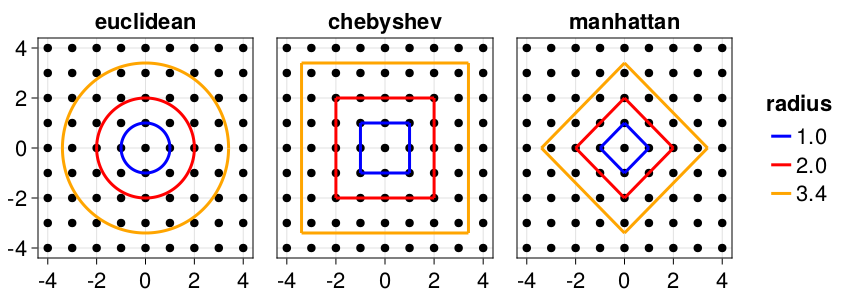
\includegraphics[width=\textwidth]{img/distance.png}
        \captionof{figure}{Esempio di metriche per il calcolo della distanza su uno spazio a griglia \cite{Agents.jl}}
        \label{fig:gridspace_distances}
    \end{minipage}

    Inoltre, è possibile utilizzare uno spazio continuo, che 
    rappresenta uno spazio di dimensione variabile con attributi di 
    posizione e velocità. Infine, esiste uno spazio misto, chiamato 
    "OpenStreetMapSpace", che rappresenta mappe come entità continue.
\end{itemize}

\subsubsection{Benchmarking e confronto con altri linguaggi}

Uno degli aspetti di maggior rilevanza nel contesto di Julia è la sua 
eccellente performance rispetto ad altri linguaggi di programmazione. 
Questo è stato dimostrato in diversi benchmark, in cui Julia ha superato 
linguaggi come Python, R e MATLAB \cite{ABAR201713} in termini di velocità 
computazionale. Questo vantaggio è particolarmente importante nelle 
simulazioni basate su agenti, in cui la velocità di esecuzione può fare 
la differenza tra la fattibilità e l'inapplicabilità di un modello.

Il confronto con Python è particolarmente rilevante, dato che Python è 
ampiamente utilizzato in campo scientifico e computazionale. Mentre 
Python offre una vasta gamma di librerie e strumenti, il suo utilizzo 
in simulazioni basate su agenti può essere limitato dalla sua lentezza. 
Julia, grazie alla sua architettura e alle sue librerie ottimizzate, 
riesce a superare questa limitazione senza compromettere la facilità 
d'uso  \cite{Flux.jl-2018} \cite{innes:2018} \cite{pal2023lux} 
\cite{rackauckas2019diffeqflux} \cite{rackauckas2020universal} 
\cite{rackauckas2017differentialequations}.

Julia è emerso come un linguaggio di programmazione di alto livello, 
versatile ed efficiente, che ha trovato applicazioni in vari campi, 
tra cui la simulazione basata su agenti. La libreria Agents.jl ha 
semplificato notevolmente lo sviluppo di modelli di simulazione basati 
su agenti in Julia, offrendo prestazioni eccezionali e una vasta gamma 
di funzionalità.

Il confronto con altri linguaggi, in particolare con Python, 
ha dimostrato che Julia può offrire un notevole vantaggio in termini 
di prestazioni computazionali, senza sacrificare la facilità d'uso e 
la versatilità.

In conclusione, Julia e la libreria Agents.jl rappresentano strumenti 
potenti per la creazione di modelli di simulazione basati su agenti che 
richiedono elevate prestazioni computazionali. La combinazione di un 
linguaggio di alto livello, come Julia, con una libreria specializzata 
come Agents.jl, offre un ambiente ideale per la progettazione e lo 
sviluppo di simulazioni avanzate in una vasta gamma di settori.

\begin{figure}[H]
    \begin{center}
        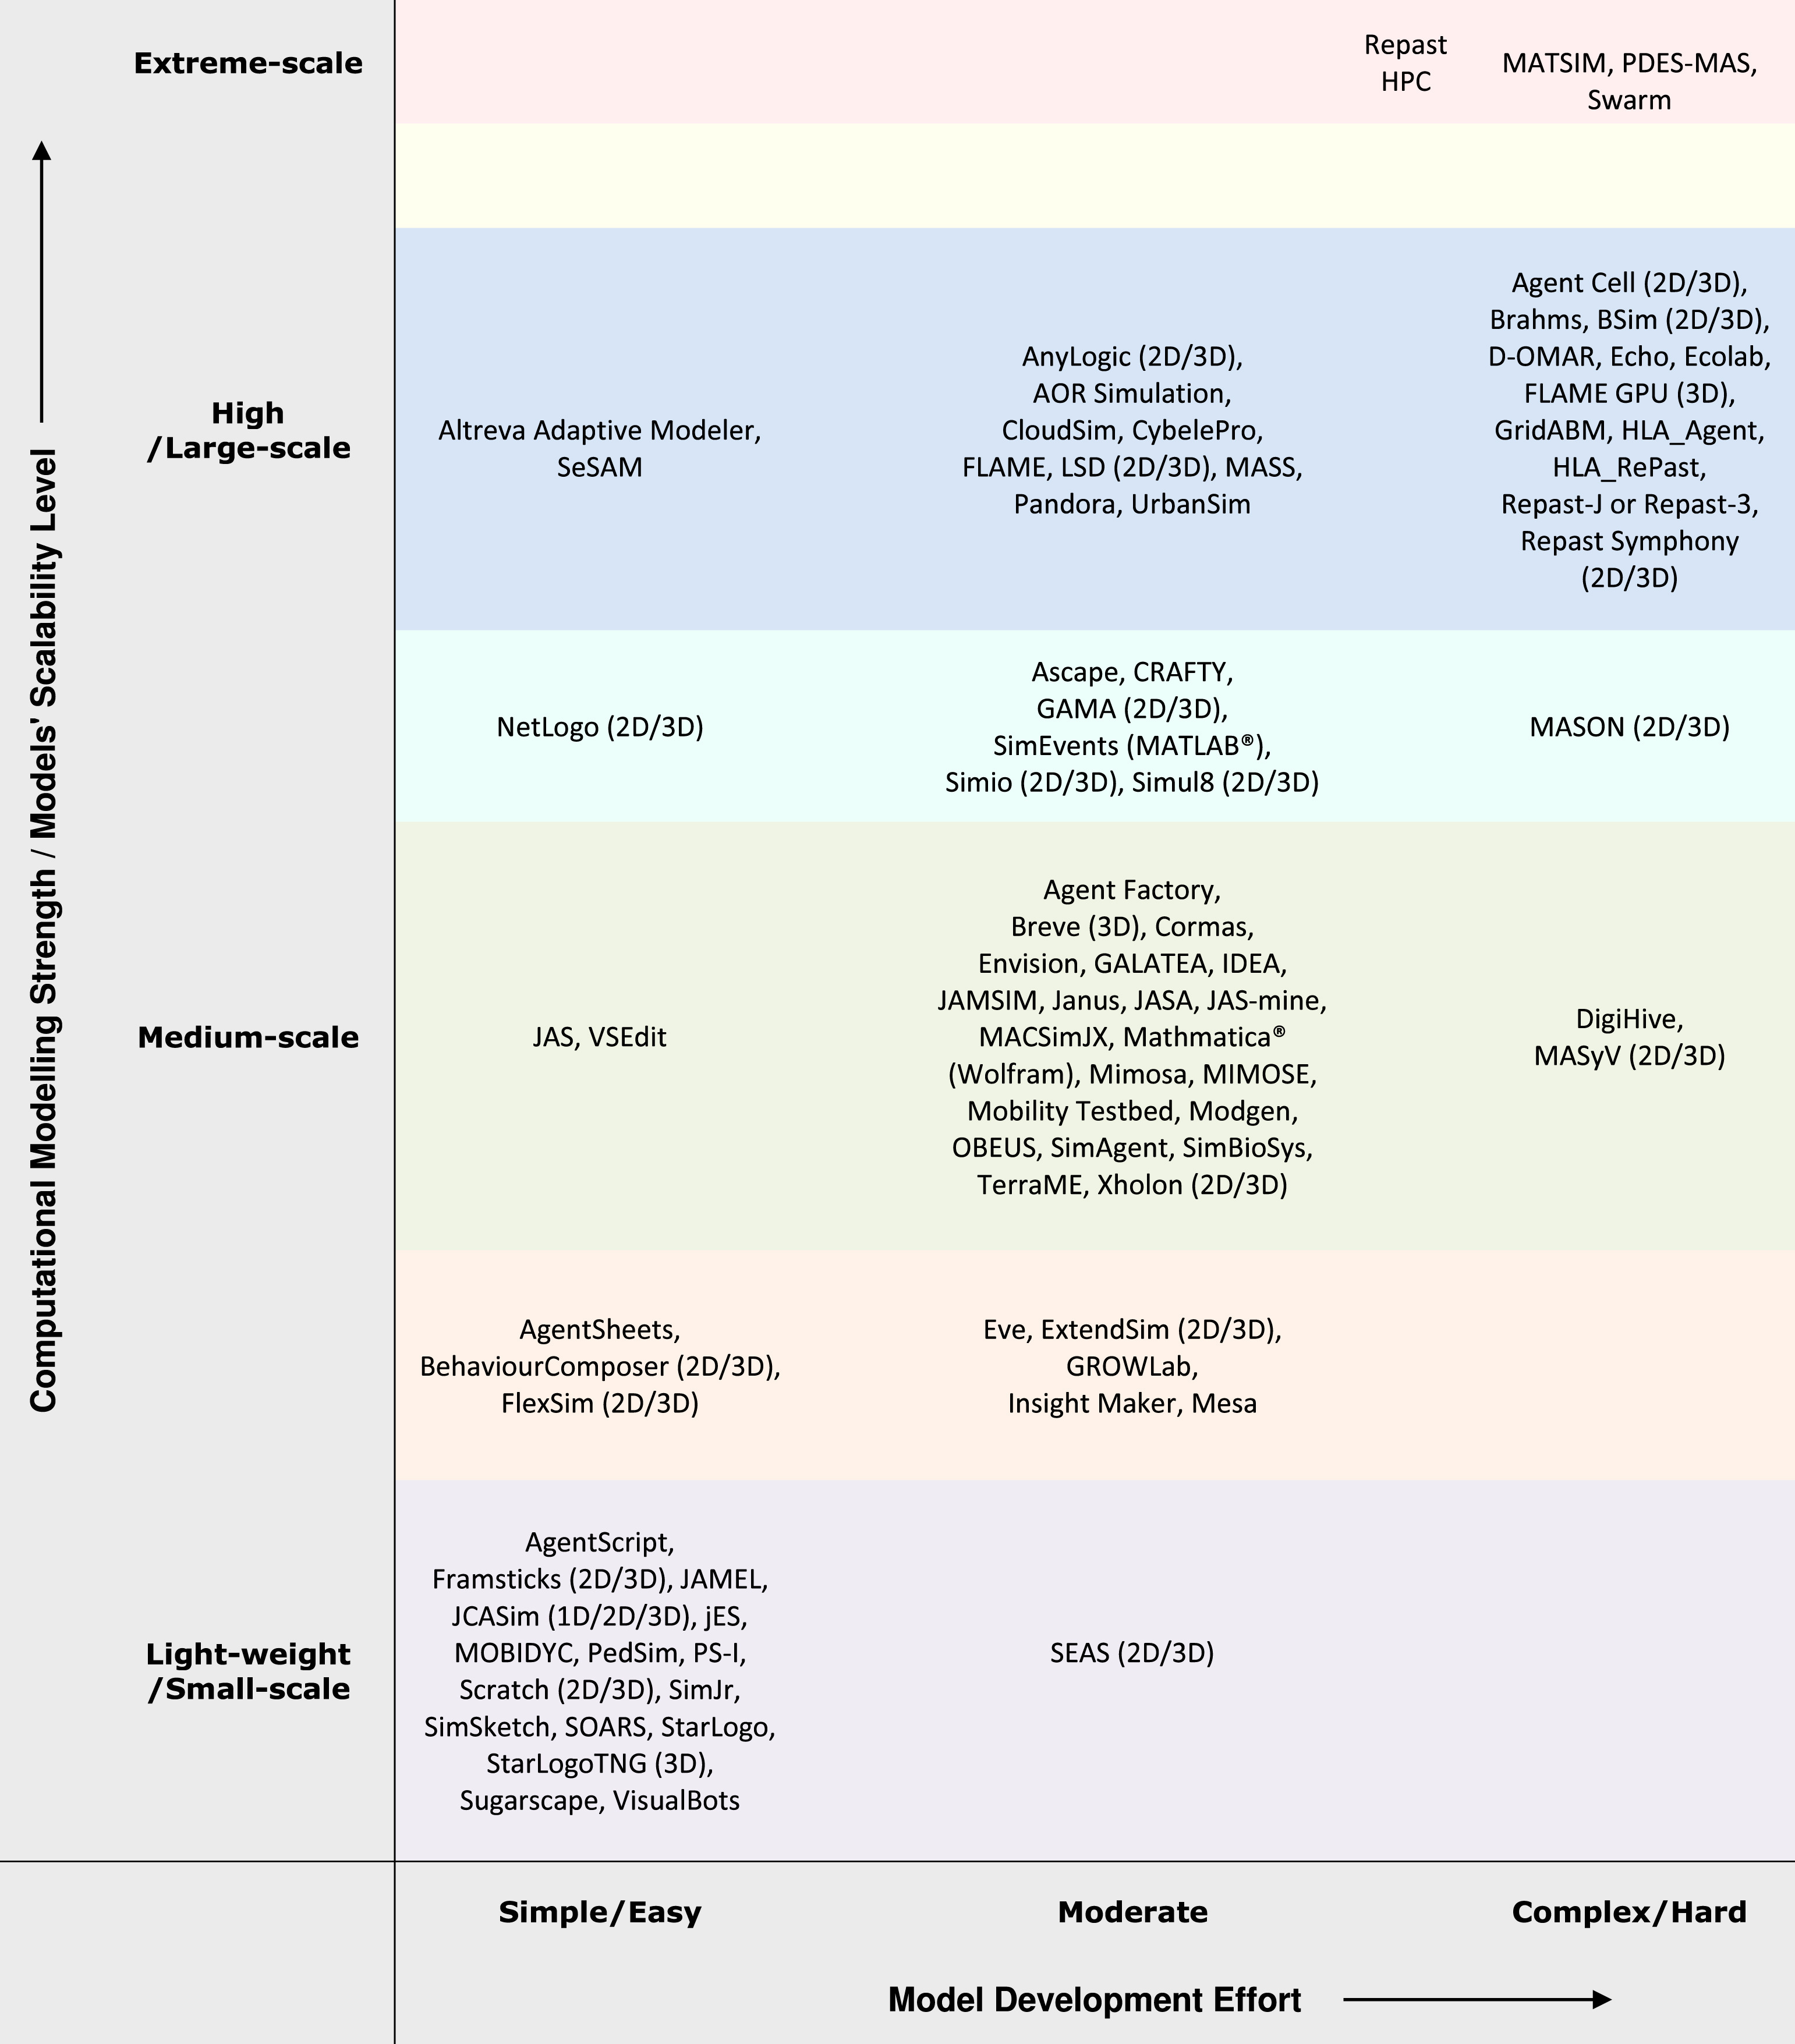
\includegraphics[width=\textwidth]{img/1-s2.0-S1574013716301198-gr1_lrg.jpg}
        \caption{Tabella comparativa \cite{ABAR201713}}
        \label{fig:Comparative_table}
    \end{center}
\end{figure}
